\providecommand{\HomA}{\mathrm{Hom}_{A}}
\providecommand{\HomB}{\mathrm{Hom}_{B}}
\providecommand{\HomC}{\mathrm{Hom}_{C}}
\providecommand{\HomOne}{\mathrm{Hom}_{1}}
\providecommand{\HomJ}{\mathrm{Hom}_{J}}
\providecommand{\colim}{\mathop{\mathrm{colim}}}
\providecommand{\qcTwo}{\mathbf{2}}

\section{虚拟装备中的形式范畴论}\label{sec:formal-category-theory-in-a-virtual-equipment}

我们对模的\trVirtualEquipment{}感兴趣的一个理由是：它把模的演算容纳于
一个\trInfinityCosmos{}之内。一个更有力的辩护则由那些可以在%
\trVirtualEquipment{}内部证明的关于∞-范畴论的定理提供。在本节中，我们
先从模论的观点重新审视\trAdjunction{}与\trFullyFaithful{}函子，然后再把
注意力转向\trInfinityCategory{}之间函子的\trLimit{}与\trColimit。

\begin{proposition}\label{prop:adjunction-counit-characterizations}
对任意一对\trFunctor{} $f\colon B\to A$ 与 $u\colon A\to B$ 以及%
\trNaturalTransformation{} $\epsilon\colon fu\Rightarrow \mathrm{id}_{A}$，
以下诸条等价：
(i) \trNaturalTransformation{} $\epsilon$ 是\trAdjunction{} $f\dashv u$ 的%
\trCounit。

(ii) 表示函子
$\ulcorner\epsilon\cdot f(-)\urcorner\colon \HomB(B,u)\to \HomA(f,A)$ 的
那个一元\trCell{}在模的\trVirtualEquipment{}中定义一个竖直同构：
\begin{center}
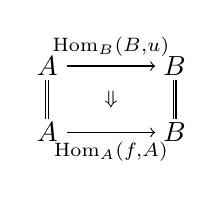
\begin{tikzpicture}[x=1em,y=1em]
  \node at (0,1.2)    {$A$};
  \node at (4.6,1.2)  {$B$};
  \node at (0,-1.2)   {$A$};
  \node at (4.6,-1.2) {$B$};
  \draw[->] (0.7,1.2)  -- node[above]{$\scriptstyle\HomB(B,u)$} (3.9,1.2);
  \draw[->] (0.7,-1.2) -- node[below]{$\scriptstyle\HomA(f,A)$} (3.9,-1.2);
  \draw[double] (0,0.7)   -- (0,-0.7);
  \draw[double] (4.6,0.7) -- (4.6,-0.7);
  \node at (2.3,0) {$\scriptstyle\Downarrow$};
\end{tikzpicture}
\end{center}
(iii) 该\trCounit{}定义一个\trExactSquare：
\begin{center}
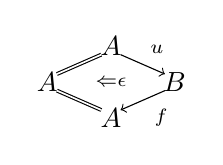
\begin{tikzpicture}[x=1em,y=1em]
  \node at (0,2.6)    {$A$};
  \node at (-2.3,1.3) {$A$};
  \node at (2.3,1.3)  {$B$};
  \node at (0,0)      {$A$};
  \draw[double,double distance=0.6pt] (-0.35,2.3) -- (-1.95,1.6);
  \draw[->] (0.35,2.3) -- node[above right,pos=0.45]{$\scriptstyle u$} (1.95,1.6);
  \draw[double,double distance=0.6pt] (-1.95,1.0) -- (-0.35,0.3);
  \draw[->] (1.95,1.0) -- node[below right,pos=0.45]{$\scriptstyle f$} (0.35,0.3);
  \node at (0,1.3) {$\scriptstyle\Leftarrow\epsilon$};
\end{tikzpicture}
\end{center}
(iv) 该\trCounit{}定义一个\textbf{绝对的}逐点右扩张图表，它被任何\trFunctor{}
$h\colon A\to C$ 所保持：
\begin{rveq}\label{eq:counit-extension-triangle}
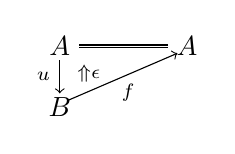
\begin{tikzpicture}[x=1em,y=1em]
  \node at (0,2.2) {$A$};
  \node at (4.6,2.2) {$A$};
  \node at (0,0) {$B$};
  \draw[double,double distance=0.6pt] (0.7,2.2) -- (3.9,2.2);
  \draw[->] (0,1.7) -- node[left]{$\scriptstyle u$} (0,0.5);
  \draw[->] (0.3,0.25) -- node[below,pos=0.55]{$\scriptstyle f$} (4.25,1.95);
  \node at (1.05,1.2) {$\scriptstyle\Uparrow\epsilon$};
\end{tikzpicture}
\end{rveq}
\end{proposition}

\begin{proof}
等价 (i)$\Leftrightarrow$(ii) 经由引理 8.1.17 由命题 4.1.1 得到证明。
说 $\epsilon\colon fu\Rightarrow \mathrm{id}_{A}$ 是正合的，即是说左下方的
二元\trCell{}是一个复合：
\begin{center}
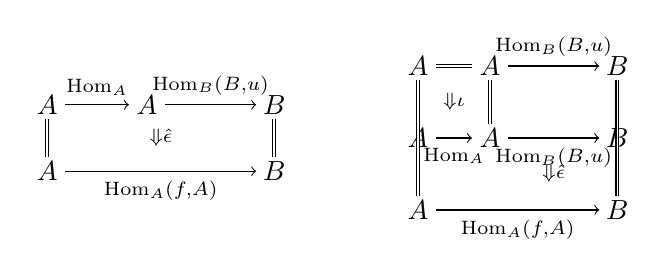
\begin{tikzpicture}[x=1em,y=1em]
  \begin{scope}
    \node at (0,1.2)   {$A$};
    \node at (3.6,1.2) {$A$};
    \node at (8.2,1.2) {$B$};
    \draw[->] (0.65,1.2) -- node[above]{$\scriptstyle\HomA$} (2.95,1.2);
    \draw[->] (4.25,1.2) -- node[above]{$\scriptstyle\HomB(B,u)$} (7.55,1.2);
    \node at (0,-1.2)    {$A$};
    \node at (8.2,-1.2)  {$B$};
    \draw[->] (0.65,-1.2) -- node[below]{$\scriptstyle\HomA(f,A)$} (7.55,-1.2);
    \draw[double] (0,0.7)   -- (0,-0.7);
    \draw[double] (8.2,0.7) -- (8.2,-0.7);
    \node at (4.1,0) {$\scriptstyle\Downarrow\hat{\epsilon}$};
  \end{scope}
  \node at (11.0,0) {$\leftrightsquigarrow$};
  \begin{scope}[shift={(13.4,0)}]
    \node at (0,2.6)   {$A$};
    \node at (2.6,2.6) {$A$};
    \node at (7.2,2.6) {$B$};
    \draw[double,double distance=0.6pt] (0.65,2.6) -- (1.95,2.6);
    \draw[->] (3.25,2.6) -- node[above]{$\scriptstyle\HomB(B,u)$} (6.55,2.6);
    \node at (0,0)   {$A$};
    \node at (2.6,0) {$A$};
    \node at (7.2,0) {$B$};
    \draw[->] (0.65,0) -- node[below]{$\scriptstyle\HomA$} (1.95,0);
    \draw[->] (3.25,0) -- node[below]{$\scriptstyle\HomB(B,u)$} (6.55,0);
    \node at (0,-2.6)  {$A$};
    \node at (7.2,-2.6){$B$};
    \draw[->] (0.65,-2.6) -- node[below]{$\scriptstyle\HomA(f,A)$} (6.55,-2.6);
    \draw[double] (0,2.1)   -- (0,-2.1);
    \draw[double] (7.2,2.1) -- (7.2,-2.1);
    \draw[double] (2.6,2.1) -- (2.6,0.5);
    \node at (1.3,1.3)  {$\scriptstyle\Downarrow\iota$};
    \node at (4.9,-1.3) {$\scriptstyle\Downarrow\hat{\epsilon}$};
  \end{scope}
\end{tikzpicture}
\end{center}
由引理 8.3.3 与引理 8.3.9(i)，这当且仅当右上方的那支一元\trCell{}是一个
复合时成立；而由引理 8.3.9(ii)，这恰好就是 (ii) 所作的断言。于是
(ii)$\Leftrightarrow$(iii)。

为证 (ii)$\Rightarrow$(iv)，我们必须证明左下方所示的这支二元\trCell{}在模的%
\trVirtualEquipment{}中定义一个右扩张图表。
\begin{center}
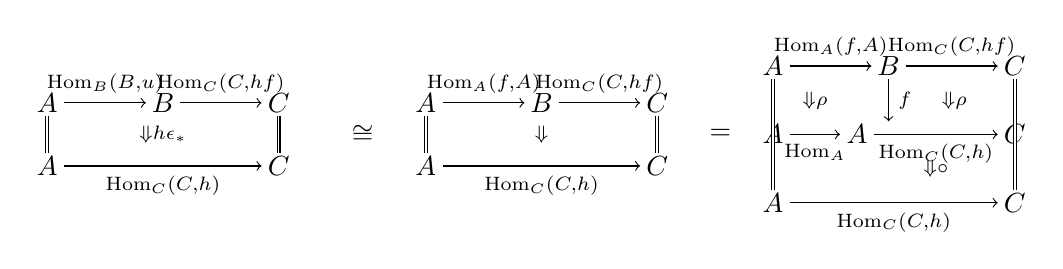
\begin{tikzpicture}[x=0.95em,y=0.95em]
  \begin{scope}
    \node at (0,1.2)   {$A$};
    \node at (4.4,1.2) {$B$};
    \node at (8.8,1.2) {$C$};
    \draw[->] (0.65,1.2)  -- node[above]{$\scriptstyle\HomB(B,u)$} (3.75,1.2);
    \draw[->] (5.05,1.2)  -- node[above]{$\scriptstyle\HomC(C,hf)$} (8.15,1.2);
    \node at (0,-1.2)  {$A$};
    \node at (8.8,-1.2){$C$};
    \draw[->] (0.65,-1.2) -- node[below]{$\scriptstyle\HomC(C,h)$} (8.15,-1.2);
    \draw[double] (0,0.7)   -- (0,-0.7);
    \draw[double] (8.8,0.7) -- (8.8,-0.7);
    \node at (4.4,0) {$\scriptstyle\Downarrow h\epsilon_{*}$};
  \end{scope}
  \node at (12.0,0) {$\cong$};
  \begin{scope}[shift={(14.4,0)}]
    \node at (0,1.2)   {$A$};
    \node at (4.4,1.2) {$B$};
    \node at (8.8,1.2) {$C$};
    \draw[->] (0.65,1.2)  -- node[above]{$\scriptstyle\HomA(f,A)$} (3.75,1.2);
    \draw[->] (5.05,1.2)  -- node[above]{$\scriptstyle\HomC(C,hf)$} (8.15,1.2);
    \node at (0,-1.2)  {$A$};
    \node at (8.8,-1.2){$C$};
    \draw[->] (0.65,-1.2) -- node[below]{$\scriptstyle\HomC(C,h)$} (8.15,-1.2);
    \draw[double] (0,0.7)   -- (0,-0.7);
    \draw[double] (8.8,0.7) -- (8.8,-0.7);
    \node at (4.4,0) {$\scriptstyle\Downarrow$};
  \end{scope}
  \node at (25.6,0) {$=$};
  \begin{scope}[shift={(27.6,0)}]
    \node at (0,2.6)   {$A$};
    \node at (4.4,2.6) {$B$};
    \node at (9.2,2.6) {$C$};
    \draw[->] (0.65,2.6)  -- node[above]{$\scriptstyle\HomA(f,A)$} (3.75,2.6);
    \draw[->] (5.05,2.6)  -- node[above]{$\scriptstyle\HomC(C,hf)$} (8.55,2.6);
    \node at (0,0)    {$A$};
    \node at (3.2,0)  {$A$};
    \node at (9.2,0)  {$C$};
    \draw[->] (0.65,0) -- node[below]{$\scriptstyle\HomA$} (2.55,0);
    \draw[->] (3.85,0) -- node[below]{$\scriptstyle\HomC(C,h)$} (8.55,0);
    \node at (0,-2.6)  {$A$};
    \node at (9.2,-2.6){$C$};
    \draw[->] (0.65,-2.6) -- node[below]{$\scriptstyle\HomC(C,h)$} (8.55,-2.6);
    \draw[double] (0,2.1)   -- (0,-2.1);
    \draw[double] (9.2,2.1) -- (9.2,-2.1);
    \draw[->] (4.4,2.1) -- node[right]{$\scriptstyle f$} (4.4,0.5);
    \node at (1.6,1.3)  {$\scriptstyle\Downarrow\rho$};
    \node at (6.9,1.3)  {$\scriptstyle\Downarrow\rho$};
    \node at (6.2,-1.3) {$\scriptstyle\Downarrow\circ$};
  \end{scope}
\end{tikzpicture}
\end{center}
由 (ii)，这个二元\trCell{}同构于中图所示形状的一个二元\trCell。\footnote{原书
中、右二图首行第二模均印作「$\HomA(A,hf)$」，按型算疑为「$\HomC(C,hf)$」
之误，此处径改。——译者注}
事实上，
引理 8.1.16 与注 8.3.13 可以用来验证：右图公式所定义的\trCell{}与竖直
同构 $\ulcorner\epsilon\cdot f(-)\urcorner\colon \HomB(B,u)\simeq \HomA(f,A)$
相复合，便产生左图的那个二元\trCell。这正是我们在\cref{lem:hom-binary-cell}
中对二元\trCell{}采用记号「$\epsilon$」的原因。于是，由%
\cref{lem:canonical-restriction-cells}，这些二元\trCell{}是模的%
\trVirtualEquipment{}中的右扩张，故可见 (ii)$\Rightarrow$(iv)。

(iv)$\Rightarrow$(i) 的证明可以完全在\trHomotopyTwoCategory{}中进行，而且不需要
「逐点的」这一形容词。事实上，这是引理 2.3.7 中留作练习 2.3.iii 的那
一部分之 op-对偶。
\end{proof}

由此可知，沿\trRightAdjoint{}的右扩张与沿\trLeftAdjoint{}的左扩张都易于
计算：

\begin{corollary}\label{cor:extensions-along-adjoints}
任何\trFunctor{}沿\trRightAdjoint{} $u\colon A\to B$ 的逐点右扩张，由其沿%
\trLeftAdjoint{} $f\colon B\to A$ 的限制给出；而任何\trFunctor{}沿一个%
\trLeftAdjoint{}的逐点左扩张，由其沿该\trRightAdjoint{}的限制给出：
\begin{center}
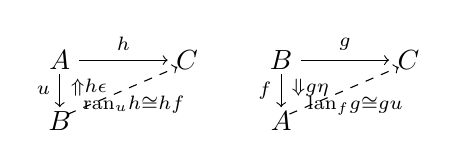
\begin{tikzpicture}[x=1em,y=1em]
  \begin{scope}
    \node at (0,2.2) {$A$};
    \node at (4.6,2.2) {$C$};
    \draw[->] (0.7,2.2) -- node[above]{$\scriptstyle h$} (3.9,2.2);
    \draw[->] (0,1.7) -- node[left]{$\scriptstyle u$} (0,0.5);
    \draw[->,dashed] (0.3,0.25) -- node[below,pos=0.6]{$\scriptstyle\mathrm{ran}_{u}h\cong hf$} (4.25,1.95);
    \node at (1.05,1.2) {$\scriptstyle\Uparrow h\epsilon$};
    \node at (0,0) {$B$};
  \end{scope}
  \begin{scope}[shift={(8.0,0)}]
    \node at (0,2.2) {$B$};
    \node at (4.6,2.2) {$C$};
    \draw[->] (0.7,2.2) -- node[above]{$\scriptstyle g$} (3.9,2.2);
    \draw[->] (0,1.7) -- node[left]{$\scriptstyle f$} (0,0.5);
    \draw[->,dashed] (0.3,0.25) -- node[below,pos=0.6]{$\scriptstyle\mathrm{lan}_{f}g\cong gu$} (4.25,1.95);
    \node at (1.05,1.2) {$\scriptstyle\Downarrow g\eta$};
    \node at (0,0) {$A$};
  \end{scope}
\end{tikzpicture}
\end{center}
\end{corollary}

\begin{proof}
在\cref{prop:adjunction-counit-characterizations}中说\trAdjunction{}
$f\dashv u$ 的\trCounit{} $\epsilon$ 是一个绝对的逐点右扩张，意即：对任何%
\trFunctor{} $h\colon A\to C$，图
\begin{center}
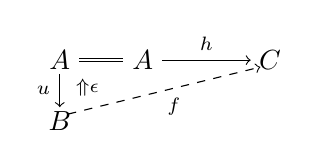
\begin{tikzpicture}[x=1em,y=1em]
  \node at (0,2.2) {$A$};
  \node at (3.0,2.2) {$A$};
  \node at (7.6,2.2) {$C$};
  \draw[double,double distance=0.6pt] (0.7,2.2) -- (2.3,2.2);
  \draw[->] (3.7,2.2) -- node[above]{$\scriptstyle h$} (6.9,2.2);
  \draw[->] (0,1.7) -- node[left]{$\scriptstyle u$} (0,0.5);
  \draw[->,dashed] (0.3,0.25) -- node[below,pos=0.55]{$\scriptstyle f$} (7.25,1.95);
  \node at (1.0,1.2) {$\scriptstyle\Uparrow\epsilon$};
  \node at (0,0) {$B$};
\end{tikzpicture}
\end{center}
是一个逐点右扩张。特别地，$hf\simeq\mathrm{ran}_{u}h$。
\end{proof}

第 3 章中的推论 3.5.6 描述了\trInfinityCategory{}之间\trFullyFaithful{}%
函子的若干等价刻画，其中一种刻画隐含地是模论的：\trFunctor{}
$k\colon A\to B$ 是\trFullyFaithful，当且仅当
$\ulcorner\mathrm{id}_{k}\urcorner\colon \qcTwo\sim \HomB(k,k)$ 是
$A\times A$ 之上的一个\trFiberedEquivalence。在模的\trVirtualEquipment{}%
中，这一条件可以用若干种方式重新表述：

\begin{lemma}\label{lem:fully-faithful-characterizations}
\trFunctor{} $k\colon A\to B$ 是\trFullyFaithful，当下列诸等价条件中的
任何一条成立时：
(i) 该方块是正合的：
\begin{center}
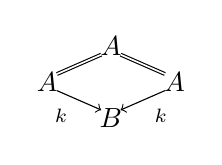
\begin{tikzpicture}[x=1em,y=1em]
  \node at (0,2.6)    {$A$};
  \node at (-2.3,1.3) {$A$};
  \node at (2.3,1.3)  {$A$};
  \node at (0,0)      {$B$};
  \draw[double,double distance=0.6pt] (-0.35,2.3) -- (-1.95,1.6);
  \draw[double,double distance=0.6pt] (0.35,2.3)  -- (1.95,1.6);
  \draw[->] (-1.95,1.0) -- node[below left,pos=0.45]{$\scriptstyle k$} (-0.35,0.3);
  \draw[->] (1.95,1.0)  -- node[below right,pos=0.45]{$\scriptstyle k$} (0.35,0.3);
\end{tikzpicture}
\end{center}
(ii) 模映射 $\ulcorner\mathrm{id}_{k}\urcorner$ 在模的\trVirtualEquipment{}%
中定义一个竖直同构：
\begin{center}
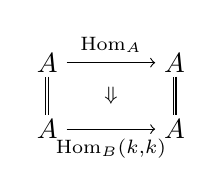
\begin{tikzpicture}[x=1em,y=1em]
  \node at (0,1.2)    {$A$};
  \node at (4.6,1.2)  {$A$};
  \node at (0,-1.2)   {$A$};
  \node at (4.6,-1.2) {$A$};
  \draw[->] (0.7,1.2)  -- node[above]{$\scriptstyle\HomA$} (3.9,1.2);
  \draw[->] (0.7,-1.2) -- node[below]{$\scriptstyle\HomB(k,k)$} (3.9,-1.2);
  \draw[double] (0,0.7)   -- (0,-0.7);
  \draw[double] (4.6,0.7) -- (4.6,-0.7);
  \node at (2.3,0) {$\scriptstyle\Downarrow$};
\end{tikzpicture}
\end{center}
\end{lemma}

\begin{proof}
在拆开诸定义之后，这一等价性由引理 8.3.9 的零元复合与一元复合、以及
引理 8.3.10 的复合关系 $\HomA\otimes\HomA\simeq\HomA$ 得出。
\end{proof}

众所周知，沿\trFullyFaithful{}函子的逐点左扩张与逐点右扩张是真正的
扩张，其意义在于：那个泛\trNaturalTransformation{}是一个同构。

\begin{proposition}[沿全忠实函子的扩张]\label{prop:extensions-along-fully-faithful}
若 $k\colon A\to B$ 是\trFullyFaithful，则对任何逐点右扩张，
\trNaturalTransformation{} $\nu\colon rk\Rightarrow f$ 是一个同构。
\begin{center}
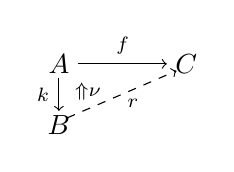
\begin{tikzpicture}[x=1em,y=1em]
  \node at (0,2.2) {$A$};
  \node at (4.6,2.2) {$C$};
  \draw[->] (0.7,2.2) -- node[above]{$\scriptstyle f$} (3.9,2.2);
  \draw[->] (0,1.7) -- node[left]{$\scriptstyle k$} (0,0.5);
  \draw[->,dashed] (0.3,0.25) -- node[below,pos=0.6]{$\scriptstyle r$} (4.25,1.95);
  \node at (1.05,1.2) {$\scriptstyle\Uparrow\nu$};
  \node at (0,0) {$B$};
\end{tikzpicture}
\end{center}
\end{proposition}

\begin{proof}
把陈述中的逐点右扩张与\cref{lem:fully-faithful-characterizations}的%
\trExactSquare{}粘贴起来，便产生一个逐点右扩张图表；它在\trHomotopyTwoCategory{}%
中的\trUniversalProperty{}可以用来构造 $\nu$ 的一个逆同构，并证明它定义
一个双侧逆：
\begin{center}
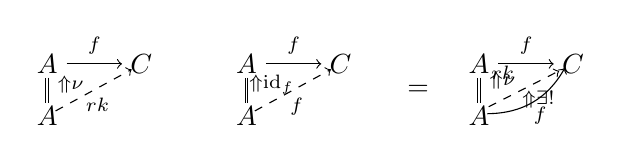
\begin{tikzpicture}[x=1em,y=1em]
  \begin{scope}
    \node at (0,1.9)   {$A$};
    \node at (3.4,1.9) {$C$};
    \node at (0,0)     {$A$};
    \draw[->] (0.7,1.9) -- node[above]{$\scriptstyle f$} (2.7,1.9);
    \draw[double] (0,1.4) -- (0,0.5);
    \draw[->,dashed] (0.3,0.2) -- node[below,pos=0.55]{$\scriptstyle rk$} (3.05,1.7);
    \node at (0.85,1.15) {$\scriptstyle\Uparrow\nu$};
  \end{scope}
  \begin{scope}[shift={(7.2,0)}]
    \node at (0,1.9)   {$A$};
    \node at (3.4,1.9) {$C$};
    \node at (0,0)     {$A$};
    \draw[->] (0.7,1.9) -- node[above]{$\scriptstyle f$} (2.7,1.9);
    \draw[double] (0,1.4) -- (0,0.5);
    \draw[->,dashed] (0.3,0.2) -- node[below,pos=0.55]{$\scriptstyle f$} (3.05,1.7);
    \node at (0.9,1.15) {$\scriptstyle\Uparrow\mathrm{id}_{f}$};
  \end{scope}
  \node at (13.4,0.95) {$=$};
  \begin{scope}[shift={(15.6,0)}]
    \node at (0,1.9)   {$A$};
    \node at (3.4,1.9) {$C$};
    \node at (0,0)     {$A$};
    \draw[->] (0.7,1.9) -- node[above]{$\scriptstyle f$} (2.7,1.9);
    \draw[double] (0,1.4) -- (0,0.5);
    \draw[->,dashed] (0.35,0.35) -- node[above left,pos=0.5]{$\scriptstyle rk$} (2.9,1.65);
    \draw[->] (0.3,0.1) to[bend right=30] node[below,pos=0.6]{$\scriptstyle f$} (3.1,1.75);
    \node at (0.85,1.3)  {$\scriptstyle\Uparrow\nu$};
    \node at (2.15,0.6)  {$\scriptstyle\Uparrow\exists!$};
  \end{scope}
\end{tikzpicture}
\end{center}
\end{proof}

\begin{proposition}\label{prop:right-adjoint-fully-faithful}
一个\trRightAdjoint{} $u\colon A\to B$ 是\trFullyFaithful，当且仅当%
\trCounit{} $\epsilon\colon fu\Rightarrow \mathrm{id}_{A}$ 是一个同构。
\end{proposition}

\begin{proof}
若 $f\dashv u$ 带有\trCounit{} $\epsilon\colon fu\Rightarrow \mathrm{id}_{A}$，
则由\cref{prop:adjunction-counit-characterizations}，\trCounit{}
$\epsilon\colon fu\Rightarrow \mathrm{id}_{A}$ 是正合的。若 $u$ 是%
\trFullyFaithful，则由\cref{lem:composites-exact-squares}，下方的复合
矩形也是正合的。
\begin{center}
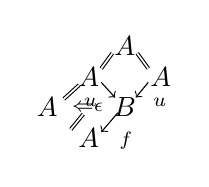
\begin{tikzpicture}[x=1em,y=1em]
  \node at (2.2,3.4)  {$A$};
  \node at (0.9,2.3)  {$A$};
  \node at (3.5,2.3)  {$A$};
  \node at (-0.6,1.2) {$A$};
  \node at (2.2,1.2)  {$B$};
  \node at (0.9,0.1)  {$A$};
  \draw[double,double distance=0.6pt] (1.75,3.15) -- (1.35,2.6);
  \draw[double,double distance=0.6pt] (2.65,3.15) -- (3.05,2.6);
  \draw[double,double distance=0.6pt] (0.55,2.0)  -- (0.0,1.5);
  \draw[double,double distance=0.6pt] (0.25,0.4)  -- (0.7,0.95);
  \draw[->] (1.35,2.1)  -- node[below left,pos=0.4]{$\scriptstyle u$} (1.85,1.55);
  \draw[->] (3.05,2.1)  -- node[below right,pos=0.4]{$\scriptstyle u$} (2.6,1.55);
  \draw[->] (1.95,1.0)  -- node[below right,pos=0.5]{$\scriptstyle f$} (1.35,0.3);
  \node at (0.85,1.2) {$\scriptstyle\Leftarrow\epsilon$};
\end{tikzpicture}
\end{center}
拆开\cref{def:exact-square}，这就是说（由引理 8.3.10 与引理 8.3.9）：
$\epsilon$ 在定义 8.4.12 的反变嵌入之下的像诱导了模的一个等价
$\epsilon^{*}\colon \HomA\simeq \HomA(fu,A)$。由命题 8.4.11，这个嵌入是%
\trFullyFaithful，从而可知 $\epsilon\colon fu\Rightarrow \mathrm{id}_{A}$
是一个同构。
反之，设 $f\dashv u$ 带有可逆的\trCounit{}%
$\epsilon\colon fu\cong\mathrm{id}_{A}$。练习 3.6.ii 与推论 4.1.3 的诸\trFiberedEquivalence
\begin{equation*}
\HomA\xrightarrow[\simeq]{\ \epsilon^{*}\ }\HomA(fu,A)
\xrightarrow[\simeq]{\ \ulcorner u(-)\cdot\eta\urcorner\ }\HomB(u,u)
\end{equation*}
复合起来，便定义了模映射 $\ulcorner\mathrm{id}_{u}\urcorner\colon \HomA\Rightarrow \HomB(u,u)$。于是，由\cref{lem:fully-faithful-characterizations}，
$u$ 是\trFullyFaithful。
\end{proof}

现在我们转向由\trInfinityCategory{}标引的图表的\trLimit{}与\trColimit。
回忆定义 1.2.23：一个\trInfinityCosmos{} $\mathcal{K}$ 是%
\trCartesianClosed，如果对任何 $J\in\mathcal{K}$ 都存在一个%
\trCosmologicalFunctor{} $(-)^{J}\colon \mathcal{K}\to\mathcal{K}$，装备有
一个\trSimplicial{}自然同构
\begin{equation*}
\mathrm{Fun}(X\times J,A)\cong \mathrm{Fun}(X,A^{J}).
\end{equation*}
由此，$A$ 中 $J$ 形图表之\trInfinityCategory{}里的\trElement{}
$f\colon 1\to A^{J}$ 双射地对应于\trInfinityCategory{}之间的\trFunctor{}
$f\colon J\to A$。在这样的上下文中，定义 2.3.8 把一个由\trInfinityCategory{}%
标引的图表 $f\colon J\to A$ 的\trLimit{}与\trColimit{}分别定义为绝对右
提升与绝对左提升：
\begin{center}
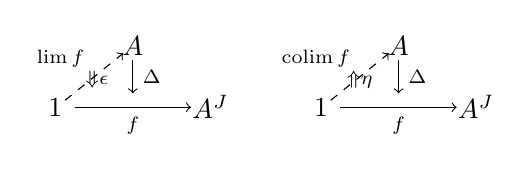
\begin{tikzpicture}[x=1em,y=1em]
  \begin{scope}
    \node at (2.8,2.2) {$A$};
    \draw[->] (2.8,1.7) -- node[right]{$\scriptstyle\Delta$} (2.8,0.5);
    \draw[->,dashed] (0.35,0.25) -- node[above left,pos=0.5]{$\scriptstyle\lim f$} (2.45,1.95);
    \node at (1.5,1.0) {$\scriptstyle\Downarrow\epsilon$};
    \node at (0,0)   {$1$};
    \node at (5.6,0) {$A^{J}$};
    \draw[->] (0.7,0) -- node[below]{$\scriptstyle f$} (4.9,0);
  \end{scope}
  \begin{scope}[shift={(9.6,0)}]
    \node at (2.8,2.2) {$A$};
    \draw[->] (2.8,1.7) -- node[right]{$\scriptstyle\Delta$} (2.8,0.5);
    \draw[->,dashed] (0.35,0.25) -- node[above left,pos=0.5]{$\scriptstyle\colim f$} (2.45,1.95);
    \node at (1.4,1.0) {$\scriptstyle\Uparrow\eta$};
    \node at (0,0)   {$1$};
    \node at (5.6,0) {$A^{J}$};
    \draw[->] (0.7,0) -- node[below]{$\scriptstyle f$} (4.9,0);
  \end{scope}
\end{tikzpicture}
\end{center}

现在我们论证：这样的\trLimit{}与\trColimit{}也可以表述为逐点%
\trKanExtension，从而把先前展开的理论拓广到那些未必\trCartesianClosed{}%
\trInfinityCosmos。

\begin{definition}\label{def:limit-colimit-diagrams}
由\trInfinityCategory{}构成的图表 $f\colon J\to A$ 的一个\textbf{\trLimit}，
由如下左图所示的一个逐点右扩张给出；而由\trInfinityCategory{}构成的图表
$f\colon J\to A$ 的一个\textbf{\trColimit}，由如下右图所示的一个逐点左
扩张给出。
\begin{center}
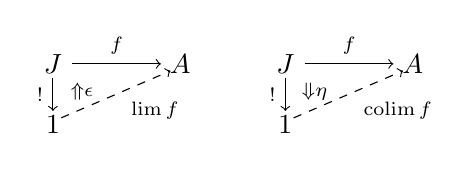
\begin{tikzpicture}[x=1em,y=1em]
  \begin{scope}
    \node at (0,2.2) {$J$};
    \node at (4.6,2.2) {$A$};
    \draw[->] (0.7,2.2) -- node[above]{$\scriptstyle f$} (3.9,2.2);
    \draw[->] (0,1.7) -- node[left]{$\scriptstyle !$} (0,0.5);
    \draw[->,dashed] (0.3,0.25) -- node[below right,pos=0.55]{$\scriptstyle\lim f$} (4.25,1.95);
    \node at (1.05,1.2) {$\scriptstyle\Uparrow\epsilon$};
    \node at (0,0) {$1$};
  \end{scope}
  \begin{scope}[shift={(8.4,0)}]
    \node at (0,2.2) {$J$};
    \node at (4.6,2.2) {$A$};
    \draw[->] (0.7,2.2) -- node[above]{$\scriptstyle f$} (3.9,2.2);
    \draw[->] (0,1.7) -- node[left]{$\scriptstyle !$} (0,0.5);
    \draw[->,dashed] (0.3,0.25) -- node[below right,pos=0.55]{$\scriptstyle\colim f$} (4.25,1.95);
    \node at (1.05,1.2) {$\scriptstyle\Downarrow\eta$};
    \node at (0,0) {$1$};
  \end{scope}
\end{tikzpicture}
\end{center}
如同定义 2.3.8 中那样，我们把\trNaturalTransformation{} $\epsilon$ 与
$\eta$ 分别称为\textbf{极限\trCone}与\textbf{余极限\trCone}。我们的第一
个任务是调和这些定义：
\end{definition}

\begin{proposition}\label{prop:limit-pointwise-extension-transpose}
在一个\trCartesianClosed{}\trInfinityCosmos{}中，任何由如下右图所示绝对
右提升图表所编码的\trLimit{}都转置而定义如下左图所示的一个逐点右扩张图表：
\begin{center}
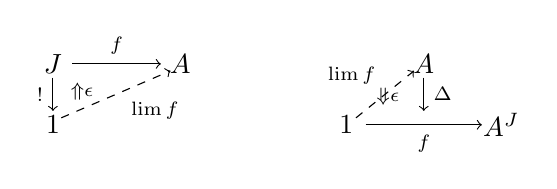
\begin{tikzpicture}[x=1em,y=1em]
  \begin{scope}
    \node at (0,2.2) {$J$};
    \node at (4.6,2.2) {$A$};
    \draw[->] (0.7,2.2) -- node[above]{$\scriptstyle f$} (3.9,2.2);
    \draw[->] (0,1.7) -- node[left]{$\scriptstyle !$} (0,0.5);
    \draw[->,dashed] (0.3,0.25) -- node[below right,pos=0.55]{$\scriptstyle\lim f$} (4.25,1.95);
    \node at (1.05,1.2) {$\scriptstyle\Uparrow\epsilon$};
    \node at (0,0) {$1$};
  \end{scope}
  \node at (8.0,1.1) {$\leftrightsquigarrow$};
  \begin{scope}[shift={(10.6,0)}]
    \node at (2.8,2.2) {$A$};
    \draw[->] (2.8,1.7) -- node[right]{$\scriptstyle\Delta$} (2.8,0.5);
    \draw[->,dashed] (0.35,0.25) -- node[above left,pos=0.5]{$\scriptstyle\lim f$} (2.45,1.95);
    \node at (1.5,1.0) {$\scriptstyle\Downarrow\epsilon$};
    \node at (0,0)   {$1$};
    \node at (5.6,0) {$A^{J}$};
    \draw[->] (0.7,0) -- node[below]{$\scriptstyle f$} (4.9,0);
  \end{scope}
\end{tikzpicture}
\end{center}
反之，任何这种形状的逐点右扩张图表都转置而定义 $A$ 中的一个\trLimit。
\end{proposition}

\begin{proof}
由\cref{lem:limit-transpose}，如下左图所示的绝对右提升图表的%
\trUniversalProperty{}转置为这样一个右扩张图表的\trUniversalProperty——
它对与\trPullback{}方块作粘贴保持稳定：
\begin{center}
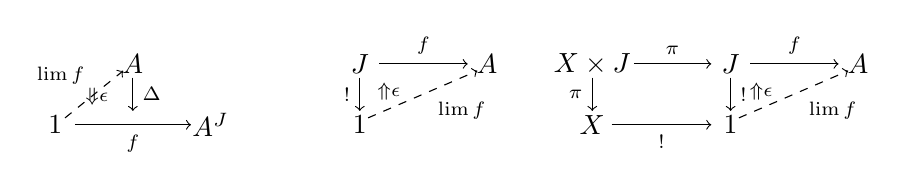
\begin{tikzpicture}[x=1em,y=1em]
  \begin{scope}
    \node at (2.8,2.2) {$A$};
    \draw[->] (2.8,1.7) -- node[right]{$\scriptstyle\Delta$} (2.8,0.5);
    \draw[->,dashed] (0.35,0.25) -- node[above left,pos=0.5]{$\scriptstyle\lim f$} (2.45,1.95);
    \node at (1.5,1.0) {$\scriptstyle\Downarrow\epsilon$};
    \node at (0,0)   {$1$};
    \node at (5.6,0) {$A^{J}$};
    \draw[->] (0.7,0) -- node[below]{$\scriptstyle f$} (4.9,0);
  \end{scope}
  \node at (8.4,1.1) {$\leftrightsquigarrow$};
  \begin{scope}[shift={(11.0,0)}]
    \node at (0,2.2) {$J$};
    \node at (4.6,2.2) {$A$};
    \draw[->] (0.7,2.2) -- node[above]{$\scriptstyle f$} (3.9,2.2);
    \draw[->] (0,1.7) -- node[left]{$\scriptstyle !$} (0,0.5);
    \draw[->,dashed] (0.3,0.25) -- node[below right,pos=0.55]{$\scriptstyle\lim f$} (4.25,1.95);
    \node at (1.05,1.2) {$\scriptstyle\Uparrow\epsilon$};
    \node at (0,0) {$1$};
  \end{scope}
  \begin{scope}[shift={(19.4,0)}]
    \node at (0,2.2)   {$X\times J$};
    \node at (5.0,2.2) {$J$};
    \node at (9.6,2.2) {$A$};
    \draw[->] (1.5,2.2) -- node[above]{$\scriptstyle\pi$} (4.3,2.2);
    \draw[->] (5.7,2.2) -- node[above]{$\scriptstyle f$} (8.9,2.2);
    \node at (0,0) {$X$};
    \node at (5.0,0) {$1$};
    \draw[->] (0,1.7) -- node[left]{$\scriptstyle\pi$} (0,0.5);
    \draw[->] (0.7,0) -- node[below]{$\scriptstyle !$} (4.3,0);
    \draw[->] (5.0,1.7) -- node[right]{$\scriptstyle !$} (5.0,0.5);
    \node at (0.9,1.5) {$\scriptstyle\lrcorner$};
    \draw[->,dashed] (5.3,0.25) -- node[below right,pos=0.55]{$\scriptstyle\lim f$} (9.25,1.95);
    \node at (6.1,1.2) {$\scriptstyle\Uparrow\epsilon$};
  \end{scope}
\end{tikzpicture}
\end{center}
由于余定义域为终\trInfinityCategory{}的余跨度上的\trCommaSquare{}归约为%
\trPullback，我们从定理 9.3.3(ii) 得知：$\epsilon\colon \Delta\lim f\Rightarrow f$
是一个绝对右提升图表，当且仅当 $\epsilon\colon \lim f\,!\Rightarrow f$ 是一个逐点右扩张。
\end{proof}

在经典\trCategory{}理论中，有一个众所周知的公式把逐点右%
\trKanExtension{}的值「逐点地」计算为\trLimit。一个对偶的余极限公式
计算逐点左 \trKanExtension。这些公式如今便可以回收过来——本质上是作为
重言式。

\begin{proposition}\label{prop:limits-from-slices}
对任何如下左图所示的逐点右扩张与任何\trElement{} $b\colon 1\to B$，
\trElement{} $rb\colon 1\to C$ 是如下右图所示图表的\trLimit：
\begin{center}
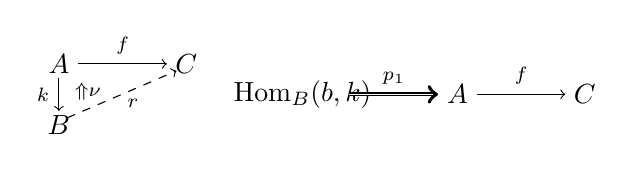
\begin{tikzpicture}[x=1em,y=1em]
  \begin{scope}
    \node at (0,2.2) {$A$};
    \node at (4.6,2.2) {$C$};
    \draw[->] (0.7,2.2) -- node[above]{$\scriptstyle f$} (3.9,2.2);
    \draw[->] (0,1.7) -- node[left]{$\scriptstyle k$} (0,0.5);
    \draw[->,dashed] (0.3,0.25) -- node[below,pos=0.6]{$\scriptstyle r$} (4.25,1.95);
    \node at (1.05,1.2) {$\scriptstyle\Uparrow\nu$};
    \node at (0,0) {$B$};
  \end{scope}
  \begin{scope}[shift={(8.8,1.1)}]
    \node at (0,0) {$\HomB(b,k)$};
    \node at (5.6,0) {$A$};
    \node at (10.2,0) {$C$};
    \draw[double,->] (1.7,0) -- node[above]{$\scriptstyle p_{1}$} (4.9,0);
    \draw[->] (6.3,0) -- node[above]{$\scriptstyle f$} (9.5,0);
  \end{scope}
\end{tikzpicture}
\end{center}
而对任何如下左图所示的逐点左扩张与任何\trElement{} $b\colon 1\to B$，
\trElement{} $\ell b\colon 1\to C$ 是如下右图所示图表的\trColimit：
\begin{center}
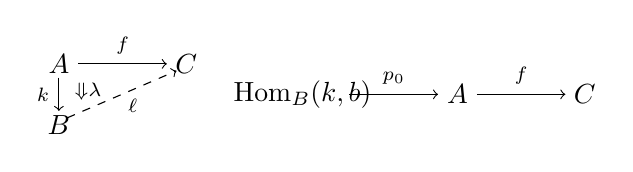
\begin{tikzpicture}[x=1em,y=1em]
  \begin{scope}
    \node at (0,2.2) {$A$};
    \node at (4.6,2.2) {$C$};
    \draw[->] (0.7,2.2) -- node[above]{$\scriptstyle f$} (3.9,2.2);
    \draw[->] (0,1.7) -- node[left]{$\scriptstyle k$} (0,0.5);
    \draw[->,dashed] (0.3,0.25) -- node[below,pos=0.6]{$\scriptstyle\ell$} (4.25,1.95);
    \node at (1.05,1.2) {$\scriptstyle\Downarrow\lambda$};
    \node at (0,0) {$B$};
  \end{scope}
  \begin{scope}[shift={(8.8,1.1)}]
    \node at (0,0) {$\HomB(k,b)$};
    \node at (5.6,0) {$A$};
    \node at (10.2,0) {$C$};
    \draw[->] (1.7,0) -- node[above]{$\scriptstyle p_{0}$} (4.9,0);
    \draw[->] (6.3,0) -- node[above]{$\scriptstyle f$} (9.5,0);
  \end{scope}
\end{tikzpicture}
\end{center}
\end{proposition}

\begin{proof}
由定理 9.3.3(ii)，复合
\begin{center}
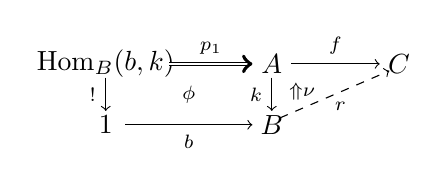
\begin{tikzpicture}[x=1em,y=1em]
  \node at (0,2.2)   {$\HomB(b,k)$};
  \node at (6.0,2.2) {$A$};
  \node at (10.6,2.2){$C$};
  \draw[double,->] (2.3,2.2) -- node[above]{$\scriptstyle p_{1}$} (5.3,2.2);
  \draw[->] (6.7,2.2) -- node[above]{$\scriptstyle f$} (9.9,2.2);
  \node at (0,0) {$1$};
  \node at (6.0,0) {$B$};
  \draw[->] (0,1.7) -- node[left]{$\scriptstyle !$} (0,0.5);
  \draw[->] (0.7,0) -- node[below]{$\scriptstyle b$} (5.3,0);
  \draw[->] (6.0,1.7) -- node[left]{$\scriptstyle k$} (6.0,0.5);
  \draw[->,dashed] (6.3,0.25) -- node[below,pos=0.55]{$\scriptstyle r$} (10.25,1.95);
  \node at (3.0,1.1) {$\scriptstyle\Nearrow\phi$};
  \node at (7.1,1.2) {$\scriptstyle\Uparrow\nu$};
\end{tikzpicture}
\end{center}
是一个逐点右扩张。由\cref{def:limit-colimit-diagrams}，这可以解释为：
$rb\colon 1\to C$ 定义了图表 $f\colon A\to C$ 沿
$p_{1}\colon \HomB(b,k)\twoheadrightarrow A$ 的限制的\trLimit。\footnote{原书印作
「$rb\colon 1\to B$」，按命题陈述与本证明（$rb\colon 1\to C$ 为所论
极限之\trElement）疑为「$1\to C$」之误，此处径改。——译者注}
\end{proof}

在定义 2.2.1 中，$A$ 中的\trInitial{}元素与\trTerminal{}元素分别定义为
唯一\trFunctor{} $!\colon A\to 1$ 的\trLeftAdjoint{}或\trRightAdjoint
\begin{center}
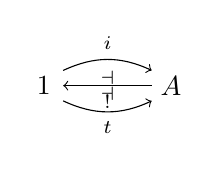
\begin{tikzpicture}[x=1em,y=1em]
  \node at (0,0)   {$1$};
  \node at (4.6,0) {$A$};
  \draw[->] (0.7,0.55) to[bend left=25] node[above]{$\scriptstyle i$} (3.9,0.55);
  \node at (2.3,0.27) {$\scriptstyle\dashv$};
  \draw[->] (3.9,0) -- node[below]{$\scriptstyle !$} (0.7,0);
  \node at (2.3,-0.3) {$\scriptstyle\dashv$};
  \draw[->] (0.7,-0.55) to[bend right=25] node[below]{$\scriptstyle t$} (3.9,-0.55);
\end{tikzpicture}
\end{center}
或者等价地（由例 2.3.10），定义为 $A^{\varnothing}\simeq 1$ 中%
\trEmptyDiagram{}的\trColimit{}或\trLimit。如例 2.3.11 中所观察到的，
一个\trInitial{}元素也可以刻画为恒同图表 $\mathrm{id}_{A}\colon A\to A$
的一个\emph{\trLimit}，而一个\trTerminal{}元素也可以刻画为其\emph{\trColimit}；我们
现在就未必\trCartesianClosed{}\trInfinityCosmos{}来证明这一点：

\begin{proposition}\label{prop:terminal-initial-elements-via-id}
对一个\trInfinityCategory{} $A$：
(i) 一个\trElement{} $t\colon 1\to A$ 是\trTerminal{}的，当且仅当它为恒同
函子 $\mathrm{id}_{A}\colon A\to A$ 定义一个\trColimit；此时，\trAdjunction{}
$!\dashv t$ 的\trUnit{}定义该余极限\trCone。
(ii) 一个\trElement{} $i\colon 1\to A$ 是\trInitial{}的，当且仅当它为恒同
函子 $\mathrm{id}_{A}\colon A\to A$ 定义一个\trLimit；此时，\trAdjunction{}
$i\dashv !$ 的\trCounit{}定义该极限\trCone。
\end{proposition}

\begin{proof}
我们证明 (ii)。由定义 2.2.1，一个\trElement{} $i\colon 1\to A$ 是%
\trInitial{}的，当且仅当它为唯一\trFunctor{} $!\colon A\to 1$ 定义一个%
\trRightAdjoint。若这一\trAdjunction{}存在，则由%
\cref{prop:adjunction-counit-characterizations}，该\trCounit{}定义一个
逐点右扩张图表
\begin{center}
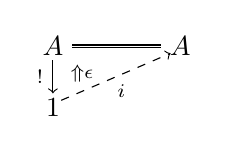
\begin{tikzpicture}[x=1em,y=1em]
  \node at (0,2.2) {$A$};
  \node at (4.6,2.2) {$A$};
  \draw[double,double distance=0.6pt] (0.7,2.2) -- (3.9,2.2);
  \draw[->] (0,1.7) -- node[left]{$\scriptstyle !$} (0,0.5);
  \draw[->,dashed] (0.3,0.25) -- node[below,pos=0.55]{$\scriptstyle i$} (4.25,1.95);
  \node at (1.05,1.2) {$\scriptstyle\Uparrow\epsilon$};
  \node at (0,0) {$1$};
\end{tikzpicture}
\end{center}
而由\cref{def:limit-colimit-diagrams}，这就把 $i$ 表达为图表
$\mathrm{id}_{A}\colon A\to A$ 的一个\trLimit。

反之，我们必须证明：一个逐点右扩张图表 $(i,\ \epsilon\colon i!\Rightarrow\mathrm{id}_{A})$
会给出一个带\trCounit{} $\epsilon$ 的\trAdjunction{}
$i\dashv !$。由引理 2.2.2，只需证明 $\epsilon i=\mathrm{id}_{i}$。由
须化的自然性（见引理 B.1.3），$\epsilon$ 与其自身的水平复合给出等式
$i!\epsilon\cdot\epsilon=\epsilon\cdot\epsilon i!$。由于\trInfinityCategory{}
$1$ 是 2-终的，$i!\epsilon=\mathrm{id}_{i!}$，于是这归约为如下粘贴等式：
\begin{center}
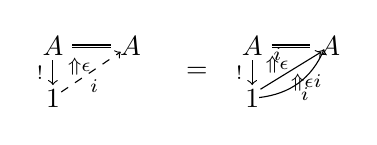
\begin{tikzpicture}[x=1em,y=1em]
  \begin{scope}
    \node at (0,1.9) {$A$};
    \node at (2.8,1.9) {$A$};
    \draw[double,double distance=0.6pt] (0.7,1.9) -- (2.1,1.9);
    \draw[->] (0,1.4) -- node[left]{$\scriptstyle !$} (0,0.5);
    \draw[->,dashed] (0.3,0.25) -- node[below,pos=0.55]{$\scriptstyle i$} (2.45,1.7);
    \node at (0.95,1.15) {$\scriptstyle\Uparrow\epsilon$};
    \node at (0,0) {$1$};
  \end{scope}
  \node at (5.2,0.95) {$=$};
  \begin{scope}[shift={(7.2,0)}]
    \node at (0,1.9) {$A$};
    \node at (2.8,1.9) {$A$};
    \draw[double,double distance=0.6pt] (0.7,1.9) -- (2.1,1.9);
    \draw[->] (0,1.4) -- node[left]{$\scriptstyle !$} (0,0.5);
    \draw[->] (0.3,0.35) -- node[above left,pos=0.5]{$\scriptstyle i$} (2.5,1.7);
    \draw[->] (0.25,0.05) to[bend right=30] node[below,pos=0.6]{$\scriptstyle i$} (2.6,1.8);
    \node at (0.9,1.25) {$\scriptstyle\Uparrow\epsilon$};
    \node at (1.95,0.6) {$\scriptstyle\Uparrow\epsilon i$};
    \node at (0,0) {$1$};
  \end{scope}
\end{tikzpicture}
\end{center}
由右扩张\trUniversalProperty{}中的唯一性陈述，即得
$\epsilon i=\mathrm{id}_{i}$，如所需。
\end{proof}

回忆定义 2.4.5：一个\trFunctor{} $k\colon I\to J$ 是\textbf{末的}
（final），如果对任何\trInfinityCategory{} $A$，方块
\begin{center}
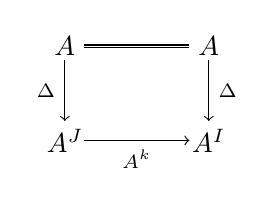
\begin{tikzpicture}[x=1em,y=1em]
  \node at (0,2.2)    {$A$};
  \node at (5.2,2.2)  {$A$};
  \node at (0,-1.2)   {$A^{J}$};
  \node at (5.2,-1.2) {$A^{I}$};
  \draw[double,double distance=0.6pt] (0.7,2.2) -- (4.5,2.2);
  \draw[->] (0,1.7) -- node[left]{$\scriptstyle\Delta$} (0,-0.5);
  \draw[->] (5.2,1.7) -- node[right]{$\scriptstyle\Delta$} (5.2,-0.5);
  \draw[->] (0.7,-1.2) -- node[below]{$\scriptstyle A^{k}$} (4.5,-1.2);
\end{tikzpicture}
\end{center}
保持并反映一切绝对左提升图表。对偶地，一个\trFunctor{} $k\colon I\to J$
是\textbf{始的}（initial），如果该方块保持并反映一切绝对右提升图表。现在
我们可以给这些概念一个更简洁的表述。

\begin{definition}\label{def:final-initial-exact-squares}
一个\trFunctor{} $k\colon I\to J$ 是\textbf{末函子}，当且仅当如下左图的
方块是正合的；是\textbf{始函子}，当且仅当如下右图的方块是正合的。
\begin{center}
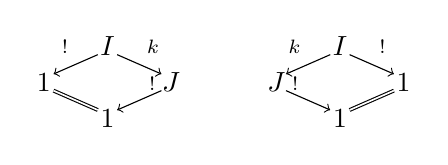
\begin{tikzpicture}[x=1em,y=1em]
  \begin{scope}
    \node at (0,2.6)    {$I$};
    \node at (-2.3,1.3) {$1$};
    \node at (2.3,1.3)  {$J$};
    \node at (0,0)      {$1$};
    \draw[->] (-0.35,2.3) -- node[above left,pos=0.45]{$\scriptstyle !$} (-1.95,1.6);
    \draw[->] (0.35,2.3)  -- node[above right,pos=0.45]{$\scriptstyle k$} (1.95,1.6);
    \draw[double,double distance=0.6pt] (-1.95,1.0) -- (-0.35,0.3);
    \draw[->] (1.95,1.0)  -- node[above right,pos=0.5]{$\scriptstyle !$} (0.35,0.3);
  \end{scope}
  \begin{scope}[shift={(8.4,0)}]
    \node at (0,2.6)    {$I$};
    \node at (-2.3,1.3) {$J$};
    \node at (2.3,1.3)  {$1$};
    \node at (0,0)      {$1$};
    \draw[->] (-0.35,2.3) -- node[above left,pos=0.45]{$\scriptstyle k$} (-1.95,1.6);
    \draw[->] (0.35,2.3)  -- node[above right,pos=0.45]{$\scriptstyle !$} (1.95,1.6);
    \draw[double,double distance=0.6pt] (1.95,1.0) -- (0.35,0.3);
    \draw[->] (-1.95,1.0) -- node[above left,pos=0.5]{$\scriptstyle !$} (-0.35,0.3);
  \end{scope}
\end{tikzpicture}
\end{center}
注意到\trFunctor{} $!\colon J\to 1$ 在右侧与在左侧分别由模
$J\xrightarrow{J}1$ 与 $1\xrightarrow{J}J$ 所表示。于是我们看到：
$k\colon I\to J$ 是末函子，当且仅当如下左图的跨度映射是模的%
\trVirtualEquipment{}中的一个复合
\begin{center}
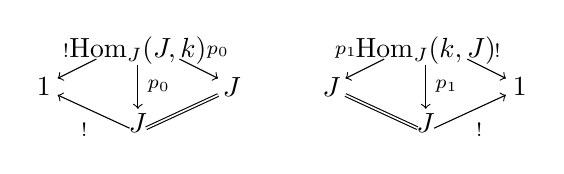
\begin{tikzpicture}[x=1em,y=1em]
  \begin{scope}
    \node at (0,2.6)    {$\HomJ(J,k)$};
    \node at (-3.4,1.3) {$1$};
    \node at (3.4,1.3)  {$J$};
    \node at (0,0)      {$J$};
    \draw[->] (-1.5,2.3) -- node[above left,pos=0.45]{$\scriptstyle !$} (-2.9,1.6);
    \draw[->] (1.5,2.3)  -- node[above right,pos=0.45]{$\scriptstyle p_{0}$} (2.9,1.6);
    \draw[->] (0,2.1) -- node[right]{$\scriptstyle p_{0}$} (0,0.5);
    \draw[->] (-0.3,-0.2) -- node[below left,pos=0.45]{$\scriptstyle !$} (-2.9,1.0);
    \draw[double,double distance=0.6pt] (0.3,-0.2) -- (2.9,1.0);
  \end{scope}
  \begin{scope}[shift={(10.4,0)}]
    \node at (0,2.6)    {$\HomJ(k,J)$};
    \node at (-3.4,1.3) {$J$};
    \node at (3.4,1.3)  {$1$};
    \node at (0,0)      {$J$};
    \draw[->] (-1.5,2.3) -- node[above left,pos=0.45]{$\scriptstyle p_{1}$} (-2.9,1.6);
    \draw[->] (1.5,2.3)  -- node[above right,pos=0.45]{$\scriptstyle !$} (2.9,1.6);
    \draw[->] (0,2.1) -- node[right]{$\scriptstyle p_{1}$} (0,0.5);
    \draw[double,double distance=0.6pt] (-0.3,-0.2) -- (-2.9,1.0);
    \draw[->] (0.3,-0.2) -- node[below right,pos=0.45]{$\scriptstyle !$} (2.9,1.0);
  \end{scope}
\end{tikzpicture}
\end{center}
而 $k\colon I\to J$ 是始函子，当且仅当如上右图的跨度映射是一个复合。
\end{definition}

\begin{remark}\label{rem:strongly-exact-finality}
如\cref{dig:strong-exactness}中所论，在 $(\infty,1)$-范畴的%
\trInfinityCosmos{}中，\trExactSquare{}自动是强正合的；此时，末函子所
满足的\trUniversalProperty{}便可以被富集。由于从 $1$ 到 $J$ 的模归约为
$J$ 上的\trDiscreteCartesianFibration，在这类上下文中，$k\colon I\to J$ 的
末性蕴涵：对每一个\trDiscreteCartesianFibration{}
$p\colon E\twoheadrightarrow J$，映射
\begin{rveq}\label{eq:final-characterization}
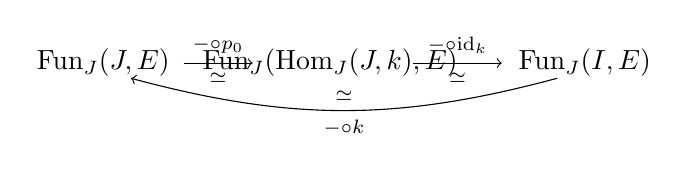
\begin{tikzpicture}[x=1em,y=1em]
  \node at (0,0)    {$\mathrm{Fun}_{J}(J,E)$};
  \node at (8.2,0)  {$\mathrm{Fun}_{J}(\HomJ(J,k),E)$};
  \node at (17.4,0) {$\mathrm{Fun}_{J}(I,E)$};
  \draw[->] (2.9,0)  -- node[above]{$\scriptstyle-\circ p_{0}$} node[below]{$\scriptstyle\simeq$} (5.4,0);
  \draw[->] (11.2,0) -- node[above]{$\scriptstyle-\circ\ulcorner\mathrm{id}_{k}\urcorner$} node[below]{$\scriptstyle\simeq$} (14.4,0);
  \draw[->] (16.4,-0.55) to[bend left=15] node[below]{$\scriptstyle-\circ k$} node[above]{$\scriptstyle\simeq$} (1.0,-0.55);
\end{tikzpicture}
\end{rveq}
是一个 Kan 复形的等价——第一个等价由强正合性给出，第二个等价由推论
5.7.19 的\trYonedaLemma{}给出。在拟范畴的\trInfinityCosmos{}中，条件
\eqref{eq:final-characterization} 刻画了拟范畴之间的末函子，Lurie 将这
一定义归于 Joyal [78, 4.1.1.1]。
\end{remark}

正如刚才所论证的，在 $(\infty,1)$-范畴的\trInfinityCosmos{}中，我们的
末函子概念蕴涵这一刻画；现在我们再论证逆方向也成立。推论 12.3.8 证明：
$(\infty,1)$-范畴的诸\trInfinityCosmos{}是强封闭的，意即：模的右扩张与
右\trLifting{}总是存在，并且满足一个表述为 Kan 复形之等价的%
\trUniversalProperty{}，而不只是在\trVirtualEquipment{}中诸\trCell{}的
一个双射。于是，由\cref{ex:closed-virtual-equipment}的强类比，
\eqref{eq:final-characterization}
对 $J$ 上的一切\trDiscreteCartesianFibration{}都定义一个等价，当且仅当%
\cref{def:final-initial-exact-squares}的方块是强正合的。因此，在拟范畴的%
\trInfinityCosmos{}中，我们的末函子概念等价于标准定义。

现在我们证明：\trLimit{}在沿始函子换指标时被保持并反映。

\begin{proposition}\label{prop:limits-along-initial-functors}
若 $k\colon I\to J$ 是始函子且 $f\colon J\to A$ 是任何图表，则 $f$ 的一个%
\trLimit{}也定义 $fk\colon I\to A$ 的一个\trLimit；反之，若 $fk\colon I\to A$
的\trLimit{}存在，则它也定义 $f\colon J\to A$ 的一个\trLimit。
\end{proposition}

\begin{proof}
由\cref{def:limit-colimit-diagrams}，$f$ 的一个\trLimit{}定义如下左图的
一个逐点右扩张；由推论 9.3.4 与\cref{def:final-initial-exact-squares}，
它又给出如下右图的另一个逐点右扩张。
\begin{center}
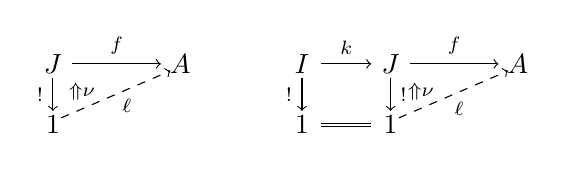
\begin{tikzpicture}[x=1em,y=1em]
  \begin{scope}
    \node at (0,2.2) {$J$};
    \node at (4.6,2.2) {$A$};
    \draw[->] (0.7,2.2) -- node[above]{$\scriptstyle f$} (3.9,2.2);
    \draw[->] (0,1.7) -- node[left]{$\scriptstyle !$} (0,0.5);
    \draw[->,dashed] (0.3,0.25) -- node[below,pos=0.6]{$\scriptstyle\ell$} (4.25,1.95);
    \node at (1.05,1.2) {$\scriptstyle\Uparrow\nu$};
    \node at (0,0) {$1$};
  \end{scope}
  \begin{scope}[shift={(9.0,0)}]
    \node at (0,2.2) {$I$};
    \node at (3.2,2.2) {$J$};
    \node at (7.8,2.2) {$A$};
    \draw[->] (0.7,2.2) -- node[above]{$\scriptstyle k$} (2.5,2.2);
    \draw[->] (3.9,2.2) -- node[above]{$\scriptstyle f$} (7.1,2.2);
    \draw[->] (0,1.7) -- node[left]{$\scriptstyle !$} (0,0.5);
    \draw[->] (3.2,1.7) -- node[right]{$\scriptstyle !$} (3.2,0.5);
    \node at (0,0)    {$1$};
    \node at (3.2,0)  {$1$};
    \draw[double,double distance=0.6pt] (0.7,0) -- (2.5,0);
    \draw[->,dashed] (3.5,0.25) -- node[below,pos=0.55]{$\scriptstyle\ell$} (7.45,1.95);
    \node at (4.3,1.2) {$\scriptstyle\Uparrow\nu$};
  \end{scope}
\end{tikzpicture}
\end{center}
由\cref{def:limit-colimit-diagrams}，这告诉我们 $\ell$ 是 $fk$ 的一个%
\trLimit。

反之，设给定一个逐点右扩张图表
\begin{center}
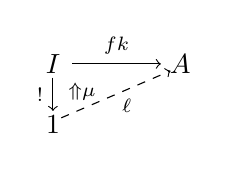
\begin{tikzpicture}[x=1em,y=1em]
  \node at (0,2.2) {$I$};
  \node at (4.6,2.2) {$A$};
  \draw[->] (0.7,2.2) -- node[above]{$\scriptstyle fk$} (3.9,2.2);
  \draw[->] (0,1.7) -- node[left]{$\scriptstyle !$} (0,0.5);
  \draw[->,dashed] (0.3,0.25) -- node[below,pos=0.6]{$\scriptstyle\ell$} (4.25,1.95);
  \node at (1.05,1.2) {$\scriptstyle\Uparrow\mu$};
  \node at (0,0) {$1$};
\end{tikzpicture}
\end{center}
由定理 9.3.3(iii)，这意味着：对从 $1$ 到 $A$ 的模的任何相容序列
$E_{1}\divideontimes\cdots\divideontimes E_{n}$，与
$\mu\colon \HomOne(1,!)\divideontimes \HomA(A,\ell)\Rightarrow \HomA(A,fk)$\footnote{原书
此模印作「$\mathrm{Hom}_{!}(1,!)$」，下标疑为「$1$」之误，此处径改。——译者注}
作复合，便在诸\trCell{}
$E_{1}\divideontimes\cdots\divideontimes E_{n}\Rightarrow \HomA(A,\ell)$
与如下左图的诸\trCell{}之间定义了一个双射：
\begin{center}
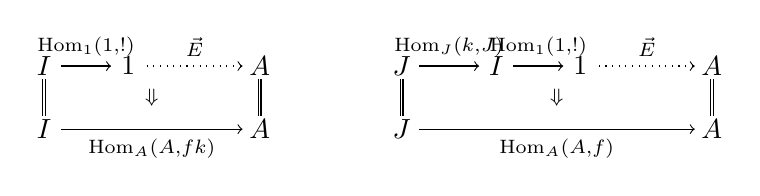
\begin{tikzpicture}[x=0.95em,y=0.95em]
  \begin{scope}
    \node at (0,1.2)   {$I$};
    \node at (3.2,1.2) {$1$};
    \node at (8.2,1.2) {$A$};
    \draw[->] (0.65,1.2)  -- node[above]{$\scriptstyle\HomOne(1,!)$} (2.55,1.2);
    \draw[->,dotted] (3.9,1.2)  -- node[above]{$\scriptstyle\vec{E}$} (7.55,1.2);
    \node at (0,-1.2)  {$I$};
    \node at (8.2,-1.2){$A$};
    \draw[->] (0.65,-1.2) -- node[below]{$\scriptstyle\HomA(A,fk)$} (7.55,-1.2);
    \draw[double] (0,0.7)   -- (0,-0.7);
    \draw[double] (8.2,0.7) -- (8.2,-0.7);
    \node at (4.1,0) {$\scriptstyle\Downarrow$};
  \end{scope}
  \node at (11.2,0) {$\leftrightsquigarrow$};
  \begin{scope}[shift={(13.6,0)}]
    \node at (0,1.2)    {$J$};
    \node at (3.6,1.2)  {$I$};
    \node at (6.8,1.2)  {$1$};
    \node at (11.8,1.2) {$A$};
    \draw[->] (0.65,1.2)  -- node[above]{$\scriptstyle\HomJ(k,J)$} (2.95,1.2);
    \draw[->] (4.25,1.2)  -- node[above]{$\scriptstyle\HomOne(1,!)$} (6.15,1.2);
    \draw[->,dotted] (7.5,1.2)  -- node[above]{$\scriptstyle\vec{E}$} (11.15,1.2);
    \node at (0,-1.2)   {$J$};
    \node at (11.8,-1.2){$A$};
    \draw[->] (0.65,-1.2) -- node[below]{$\scriptstyle\HomA(A,f)$} (11.15,-1.2);
    \draw[double] (0,0.7)    -- (0,-0.7);
    \draw[double] (11.8,0.7) -- (11.8,-0.7);
    \node at (5.9,0) {$\scriptstyle\Downarrow$};
  \end{scope}
\end{tikzpicture}
\end{center}
由推论 8.4.6，左图的诸\trCell{}与右图的诸\trCell{}处于双射之中。

说 $k\colon I\to J$ 是始函子，据\cref{def:final-initial-exact-squares}，
意即：由恒同所诱导的、从 $J$ 到 $1$ 的模的映射
$\HomJ(k,J)\divideontimes \HomOne(1,!)\Rightarrow \HomOne(1,!)$ 是一个复合。
于是，右图的诸\trCell{}与如下形状的诸\trCell{}处于双射之中：
\begin{center}
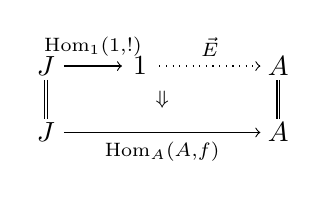
\begin{tikzpicture}[x=1em,y=1em]
  \node at (0,1.2)   {$J$};
  \node at (3.4,1.2) {$1$};
  \node at (8.4,1.2) {$A$};
  \draw[->] (0.65,1.2)  -- node[above]{$\scriptstyle\HomOne(1,!)$} (2.75,1.2);
  \draw[->,dotted] (4.1,1.2)  -- node[above]{$\scriptstyle\vec{E}$} (7.75,1.2);
  \node at (0,-1.2)  {$J$};
  \node at (8.4,-1.2){$A$};
  \draw[->] (0.65,-1.2) -- node[below]{$\scriptstyle\HomA(A,f)$} (7.75,-1.2);
  \draw[double] (0,0.7)   -- (0,-0.7);
  \draw[double] (8.4,0.7) -- (8.4,-0.7);
  \node at (4.2,0) {$\scriptstyle\Downarrow$};
\end{tikzpicture}
\end{center}

这一复合双射断言：对应于模恒同胞腔 $\mathrm{id}\colon \HomA(A,\ell)\Rightarrow\HomA(A,\ell)$ 的\trCell{}
$\nu\colon \HomOne(1,!)\divideontimes \HomA(A,\ell)\Rightarrow \HomA(A,f)$，
把 $1\xrightarrow{\HomA(A,\ell)}A$ 显示为 $J\xrightarrow{\HomA(A,f)}A$
沿 $J\xrightarrow{\HomOne(1,!)}1$ 的右扩张。拆开定义 $\nu$ 的那些双射，
我们看到 $\nu k=\mu$。于是 $\nu\colon \ell!\Rightarrow f$ 是一个逐点右
扩张，而由\cref{prop:limit-pointwise-extension-transpose}我们得出结论：
$\ell\colon 1\to A$ 定义 $f\colon J\to A$ 的一个\trLimit，如所需。
\end{proof}

尚待完成的是把定理 2.4.2——右伴随保持\trLimit{}而左伴随保持%
\trColimit——拓广到由一般\trInfinityCosmos{}中的\trInfinityCategory{}%
标引的图表。在定理 9.5.7 中，我们将证明这一结果的一个推广，它覆盖由一支
模加权的\trLimit{}与\trColimit，其意义我们即将引入。

\subsection*{练习}

\begin{exercise}\label{ex:unit-exact-square}
证明：\trAdjunction{} $f\dashv u$ 的\trUnit{}定义一个\trExactSquare：
\begin{center}
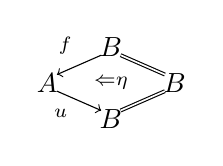
\begin{tikzpicture}[x=1em,y=1em]
  \node at (0,2.6)    {$B$};
  \node at (-2.3,1.3) {$A$};
  \node at (2.3,1.3)  {$B$};
  \node at (0,0)      {$B$};
  \draw[->] (-0.35,2.3) -- node[above left,pos=0.45]{$\scriptstyle f$} (-1.95,1.6);
  \draw[double,double distance=0.6pt] (0.35,2.3) -- (1.95,1.6);
  \draw[->] (-1.95,1.0) -- node[below left,pos=0.45]{$\scriptstyle u$} (-0.35,0.3);
  \draw[double,double distance=0.6pt] (1.95,1.0) -- (0.35,0.3);
  \node at (0,1.3) {$\scriptstyle\Leftarrow\eta$};
\end{tikzpicture}
\end{center}
\end{exercise}

\begin{exercise}\label{ex:mate-exact-square}
证明：任何如下左图所示、涉及平行伴随 $f\dashv u$ 与 $k\dashv r$ 的方块
$\alpha$，只要其对应（mate）定义一个同构，便是正合的。
\begin{center}
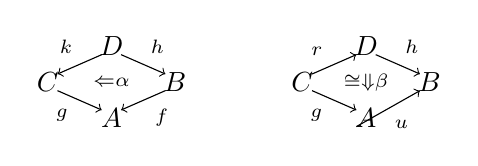
\begin{tikzpicture}[x=1em,y=1em]
  \begin{scope}
    \node at (0,2.6)    {$D$};
    \node at (-2.3,1.3) {$C$};
    \node at (2.3,1.3)  {$B$};
    \node at (0,0)      {$A$};
    \draw[->] (-0.35,2.3) -- node[above left,pos=0.45]{$\scriptstyle k$} (-1.95,1.6);
    \draw[->] (0.35,2.3)  -- node[above right,pos=0.45]{$\scriptstyle h$} (1.95,1.6);
    \draw[->] (-1.95,1.0) -- node[below left,pos=0.45]{$\scriptstyle g$} (-0.35,0.3);
    \draw[->] (1.95,1.0)  -- node[below right,pos=0.45]{$\scriptstyle f$} (0.35,0.3);
    \node at (0,1.3) {$\scriptstyle\Leftarrow\alpha$};
  \end{scope}
  \node at (5.6,1.3) {$\leftrightsquigarrow$};
  \begin{scope}[shift={(9.2,0)}]
    \node at (0,2.6)    {$D$};
    \node at (-2.3,1.3) {$C$};
    \node at (2.3,1.3)  {$B$};
    \node at (0,0)      {$A$};
    \draw[->] (-1.95,1.6) -- node[above left,pos=0.45]{$\scriptstyle r$} (-0.35,2.3);
    \draw[->] (0.35,2.3)  -- node[above right,pos=0.45]{$\scriptstyle h$} (1.95,1.6);
    \draw[->] (-1.95,1.0) -- node[below left,pos=0.45]{$\scriptstyle g$} (-0.35,0.3);
    \draw[->] (-0.35,-0.3) -- node[below right,pos=0.45]{$\scriptstyle u$} (1.95,1.0);
    \node at (0,1.3)  {$\scriptstyle\cong\Downarrow\beta$};
  \end{scope}
\end{tikzpicture}
\end{center}
\end{exercise}

\begin{exercise}\label{ex:right-adjoint-final-square}
证明：若 $k\colon I\to J$ 是一个\trRightAdjoint，则方块
\begin{center}
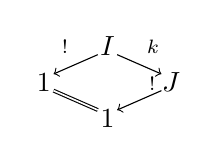
\begin{tikzpicture}[x=1em,y=1em]
  \node at (0,2.6)    {$I$};
  \node at (-2.3,1.3) {$1$};
  \node at (2.3,1.3)  {$J$};
  \node at (0,0)      {$1$};
  \draw[->] (-0.35,2.3) -- node[above left,pos=0.45]{$\scriptstyle !$} (-1.95,1.6);
  \draw[->] (0.35,2.3)  -- node[above right,pos=0.45]{$\scriptstyle k$} (1.95,1.6);
  \draw[double,double distance=0.6pt] (-1.95,1.0) -- (-0.35,0.3);
  \draw[->] (1.95,1.0)  -- node[above right,pos=0.5]{$\scriptstyle !$} (0.35,0.3);
\end{tikzpicture}
\end{center}
是正合的，从而重新证明命题 2.4.6。
\end{exercise}

